% ============================================================================
% Lecture 15 (B14): Krusell--Smith and Young's Method
% Deep Learning for Solving and Estimating Dynamic Models in Economics and Finance
% Course author: Simon Scheidegger
% ============================================================================

\documentclass[aspectratio=169,11pt]{beamer}

% ---------- Theme and colors ----------
\usecolortheme{dove}
\setbeamertemplate{navigation symbols}{}
\setbeamertemplate{footline}{%
  \hfill\usebeamerfont{page number in head/foot}%
  \usebeamercolor[fg]{normal text}%
  \insertframenumber\,/\,\inserttotalframenumber\kern1em\vskip4pt}
\setbeamerfont{frametitle}{size=\huge}

% ---------- Packages ----------
\usepackage[utf8]{inputenc}
\usepackage[T1]{fontenc}
\usepackage{lmodern}
\usepackage{amsmath,amssymb,amsfonts}
\usepackage{bm}
\usepackage{graphicx}
\usepackage{tikz}
\usetikzlibrary{shapes,arrows.meta,positioning,calc,fit,backgrounds,patterns,decorations.pathreplacing}
\usepackage{pgfplots}
\pgfplotsset{compat=1.18}
\usepackage{booktabs}
\usepackage{hyperref}
\usepackage{multicol}
\usepackage{xcolor}
\usepackage{algorithm}
\usepackage{algorithmic}
\usepackage{listings}

% ---------- Listings style for Python ----------
\lstset{
    language=Python,
    basicstyle=\small\ttfamily,
    keywordstyle=\color{uzhblue}\bfseries,
    commentstyle=\color{uzhgreydark}\itshape,
    stringstyle=\color{darkgreen},
    showstringspaces=false,
    breaklines=true,
    frame=none,
    xleftmargin=0pt,
    aboveskip=4pt,
    belowskip=4pt,
    escapeinside={(*@}{@*)},
}

% ---------- Custom colors ----------
\definecolor{uzhblue}{rgb}{0,0,0.5}
\definecolor{uzhgreylight}{RGB}{236,238,241}
\definecolor{uzhgreydark}{RGB}{81,86,94}
\definecolor{harvardcrimson}{RGB}{153,0,0}
\definecolor{unil@blue}{RGB}{0,140,204}
\definecolor{unil@black}{RGB}{35,31,32}
\definecolor{darkgreen}{RGB}{0,100,0}
\definecolor{darkred}{RGB}{139,0,0}
\definecolor{softblue}{RGB}{70,130,180}
\definecolor{softorange}{RGB}{230,159,0}
\definecolor{softgreen}{RGB}{0,158,115}

% ---------- Set beamer colors ----------
\setbeamercolor{frametitle}{bg=uzhgreylight, fg=uzhblue}
\setbeamercolor{title}{fg=uzhblue}
\setbeamercolor{structure}{fg=uzhblue}
\setbeamercolor{block title}{bg=unil@blue, fg=white}
\setbeamercolor{block body}{bg=uzhgreylight}
\setbeamercolor{block title alerted}{bg=darkred,fg=white}
\setbeamercolor{block body alerted}{bg=red!5}
\setbeamercolor{block title example}{bg=darkgreen,fg=white}
\setbeamercolor{block body example}{bg=green!5}
\setbeamercolor{item}{fg=unil@black}
\setbeamercolor{normal text}{fg=unil@black}

% ---------- Emphasis and hyperlinks ----------
\newcommand{\emphc}[1]{\textcolor{harvardcrimson}{#1}}
\hypersetup{colorlinks,linkcolor=harvardcrimson,urlcolor=harvardcrimson}

% ---------- Math commands ----------
\newcommand{\x}{\bm{x}}
\newcommand{\w}{\bm{w}}
\newcommand{\bb}{\bm{b}}
\newcommand{\z}{\bm{z}}
\newcommand{\W}{\bm{W}}
\newcommand{\X}{\bm{X}}
\renewcommand{\a}{\bm{a}}
\newcommand{\R}{\mathbb{R}}
\newcommand{\E}[1]{\mathbb{E}\!\left[#1\right]}
\DeclareMathOperator*{\argmin}{arg\,min}
\DeclareMathOperator*{\argmax}{arg\,max}

% ---------- Title ----------
\title[Lecture 16 (B15)]{Lecture 16 (B15): Continuum-Agent DEQNs --- Method Comparison}
\subtitle{DEQN with histogram encoding, DeepHAM, all-in-one DL, head-to-head}
\author{Simon Scheidegger}
\institute{HEC, University of Lausanne}
\date{}
\begin{document}

% Custom command used in some "Finger Exercise" frame titles.
\providecommand{\exercisepause}{%
  \tikz[baseline=(X.base)]{\node[fill=darkgreen!80!black, text=white,
  rounded corners=2pt, inner sep=3pt, font=\scriptsize\bfseries](X){PAUSE};}}

{\setbeamercolor{background canvas}{bg=uzhgreylight}
\begin{frame}
\titlepage
\end{frame}
}

% --- About-this-lecture orientation ---
\begin{frame}{About this lecture}
\small
\begin{block}{What this lecture covers}
\begin{itemize}\itemsep2pt
  \item Embedding Young's method inside a DEQN training loop
  \item Three deep-learning recipes for KS: all-in-one, DeepHAM, histogram-DEQN
  \item Head-to-head: when to use which architecture
\end{itemize}
\end{block}
\begin{block}{Builds on}
\begin{itemize}\itemsep2pt
  \item Lecture 15 (Young's method, traditional KS)
\end{itemize}
\end{block}
\begin{block}{Leads to}
\begin{itemize}\itemsep2pt
  \item Lecture 17 (sequence-space DEQNs)
  \item Lecture 20+ (continuous-time HA)
\end{itemize}
\end{block}
\end{frame}

\begin{frame}{Architecture Comparison: Traditional KS vs.\ DEQN}
\vspace{-0.3em}
\begin{columns}[T]
\column{0.48\textwidth}
\begin{center}
\textbf{Traditional KS}\\[2pt]
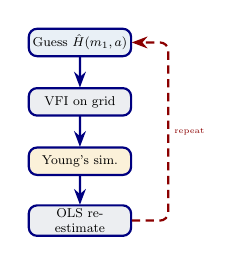
\begin{tikzpicture}[scale=0.58, every node/.style={transform shape},
    box/.style={rectangle, draw=uzhblue, thick, fill=uzhgreylight,
        minimum width=2.2cm, minimum height=0.6cm, font=\footnotesize,
        rounded corners=3pt, inner sep=2pt, text width=2.1cm, align=center},
    arr/.style={-{Stealth[length=2mm]}, thick, uzhblue}
]
    \node[box, fill=softblue!12] (fc) at (0,4.2) {Guess $\hat{H}(m_1,a)$};
    \node[box] (vfi) at (0,2.9) {VFI on grid};
    \node[box, fill=softorange!15] (sim) at (0,1.6) {Young's sim.};
    \node[box] (ols) at (0,0.3) {OLS re-estimate};

    \draw[arr] (fc) -- (vfi);
    \draw[arr] (vfi) -- (sim);
    \draw[arr] (sim) -- (ols);
    \draw[arr, darkred, densely dashed, rounded corners=3pt]
        (ols.east) -- ++(0.8,0) |- (fc.east)
        node[pos=0.25, right, font=\tiny, darkred] {repeat};
\end{tikzpicture}
\end{center}
{\scriptsize Outer loop; policy sees $m_1$ only; grid-based VFI.}

\column{0.48\textwidth}
\begin{center}
\textbf{DEQN + Young's}\\[2pt]
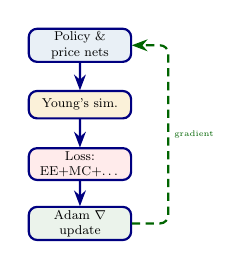
\begin{tikzpicture}[scale=0.58, every node/.style={transform shape},
    box/.style={rectangle, draw=uzhblue, thick, fill=uzhgreylight,
        minimum width=2.2cm, minimum height=0.6cm, font=\footnotesize,
        rounded corners=3pt, inner sep=2pt, text width=2.1cm, align=center},
    arr/.style={-{Stealth[length=2mm]}, thick, uzhblue}
]
    \node[box, fill=softblue!12] (nn) at (0,4.2) {Policy \& price nets};
    \node[box, fill=softorange!15] (young) at (0,2.9) {Young's sim.};
    \node[box, fill=red!8] (loss) at (0,1.6) {Loss: EE+MC+\ldots};
    \node[box, fill=darkgreen!8] (adam) at (0,0.3) {Adam $\nabla$ update};

    \draw[arr] (nn) -- (young);
    \draw[arr] (young) -- (loss);
    \draw[arr] (loss) -- (adam);
    \draw[arr, darkgreen, densely dashed, rounded corners=3pt]
        (adam.east) -- ++(0.8,0) |- (nn.east)
        node[pos=0.25, right, font=\tiny, darkgreen] {gradient};
\end{tikzpicture}
\end{center}
{\scriptsize Single loop; policy sees \emphc{full histogram}; differentiable.}
\end{columns}

\vspace{-0.1em}
\begin{center}
\scriptsize
\begin{tabular}{lcc}
\toprule
& \textbf{Traditional KS} & \textbf{DEQN} \\
\midrule
Distribution info & mean $m_1$ only & \emphc{full histogram} \\
Forecasting rule & hand-specified & \emphc{learned (price net)} \\
Outer loop & implementation-dependent & \emphc{none} \\
Policy solver & VFI on grid & \emphc{neural network} \\
\bottomrule
\end{tabular}
\end{center}
\end{frame}

% --- Slide 40: Model Specification ---
\begin{frame}{Teaching Model Specification (DEQN Version)}
\small
\textbf{Bewley endowment economy} (Azinovic et al.\ 2022, Appendix A.5):

\vspace{0.1em}
\begin{columns}[T]
\column{0.49\textwidth}
\scriptsize
\begin{center}
\renewcommand{\arraystretch}{1.1}
\begin{tabular}{ll}
\toprule
\textbf{Component} & \textbf{Value} \\
\midrule
Preferences (EZ) & $\beta=0.95$, $\rho=2$, $\sigma=8$ \\
Asset & Bonds, unit net supply \\
Idiosyncratic $\eta$ & $\{0.8,1.2\}$, $\Pi_\eta=\bigl(\begin{smallmatrix}0.7&0.3\\0.3&0.7\end{smallmatrix}\bigr)$ \\
Aggregate shocks & 6 states ($2{\times}3$) \\
Asset grid & $N_b=100$, $b\in[0,20]$ \\
Borrowing & $b_{t+1}\geq 0$ \\
\bottomrule
\end{tabular}
\end{center}
Budget: $c_t + p_t b_{t+1} = b_t + \eta_t w(a_t)$

\column{0.46\textwidth}
\begin{block}{Aggregate Shocks ($n_Z=6$)}
\footnotesize
\renewcommand{\arraystretch}{1.0}
\begin{tabular}{cccc}
\toprule
$a_t$ & Uncert. & Income & $Y(a_t)$ \\
\midrule
0 & Low  & Low  & 0.95 \\
1 & Low  & Mid  & 1.00 \\
2 & Low  & High & 1.05 \\
3 & High & Low  & 0.95 \\
4 & High & Mid  & 1.00 \\
5 & High & High & 1.05 \\
\bottomrule
\end{tabular}
\vspace{1pt}
{\tiny Persistence $=0.8$; product-form transition matrix.}
\end{block}
\end{columns}
\end{frame}

% --- Slide 41: Bridge from Notebook 10 ---
\begin{frame}{Bridge: From Notebook 10 to Notebook 11}
\footnotesize
\begin{center}
\renewcommand{\arraystretch}{1.08}
\begin{tabular}{@{}p{0.25\textwidth}p{0.26\textwidth}p{0.31\textwidth}@{}}
\toprule
\textbf{Concept} & \textbf{Notebook 10} & \textbf{Notebook 11} \\
\midrule
Individual asset & scalar $w$ or $k$ & bond holdings $b$ \\
Distribution & one histogram $h(k)$ & two histograms $(h^{0.8}, h^{1.2})$ \\
Policy input & hand-set rule $g(k)$ & NN policy $b'(\eta,b,x_t^{agg})$ \\
One forward step & redistribute mass once & \texttt{get\_weights\_eta()} update \\
Aggregation & weighted mean & histogram dot product $\mathbf{h}_t \cdot \mathbf{b}'$ \\
\bottomrule
\end{tabular}
\end{center}

\vspace{0.2em}
\begin{alertblock}{Reading order}
Read \texttt{10\_Youngs\_Method\_Examples} first for the operator, then \texttt{11\_Continuum\_of\_Agents\_DEQN} for the same operator inside the DEQN state vector and loss.
\end{alertblock}
\end{frame}

% --- Slide 42: State Space with Histogram Encoding ---
\begin{frame}{State Space with Histogram Encoding}
\textbf{Key innovation:} encode $\mu_t$ as a histogram on $N_b$ grid points.

\vspace{0.3em}
\begin{center}
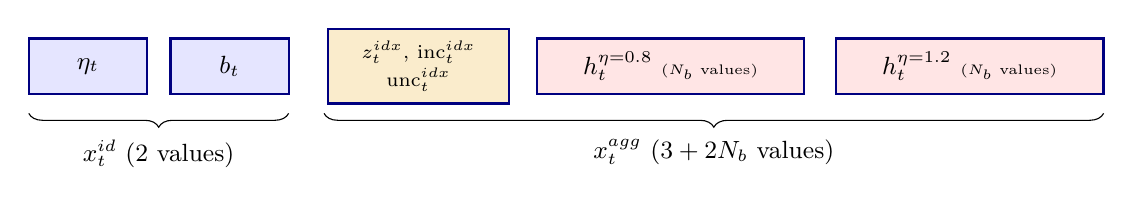
\begin{tikzpicture}[
    seg/.style={rectangle, draw=uzhblue, thick, minimum height=0.7cm, font=\small,
        inner sep=3pt},
    arr/.style={-{Stealth[length=2.5mm]}, thick, uzhblue}
]
    % Individual state
    \node[seg, fill=blue!10, minimum width=1.5cm] (eta) at (0,0) {$\eta_t$};
    \node[seg, fill=blue!10, minimum width=1.5cm] (b) at (1.8,0) {$b_t$};

    % Aggregate state
    \node[seg, fill=softorange!20, minimum width=2.3cm] (a) at (4.2,0)
        {\begin{tabular}{c}\scriptsize $z_t^{idx},\,\mathrm{inc}_t^{idx}$\\[-1pt]\scriptsize $\mathrm{unc}_t^{idx}$\end{tabular}};
    \node[seg, fill=red!10, minimum width=3.4cm] (h1) at (7.4,0) {$h_t^{\eta=0.8}$ {\tiny ($N_b$ values)}};
    \node[seg, fill=red!10, minimum width=3.4cm] (h2) at (11.2,0) {$h_t^{\eta=1.2}$ {\tiny ($N_b$ values)}};

    % Braces
    \draw[decorate, decoration={brace, amplitude=5pt, mirror}] (-0.75,-0.6) -- (2.55,-0.6)
        node[midway, below=6pt, font=\small] {$x_t^{id}$ (2 values)};
    \draw[decorate, decoration={brace, amplitude=5pt, mirror}] (3.0,-0.6) -- (12.9,-0.6)
        node[midway, below=6pt, font=\small] {$x_t^{agg}$ ($3 + 2 N_b$ values)};
\end{tikzpicture}
\end{center}

\vspace{0.5em}
\[
\boxed{\text{Total input dimension} = \underbrace{2}_{\text{individual}} + \underbrace{3 + 2 N_b}_{\text{aggregate}} = 5 + 2 N_b}
\]

\vspace{0.3em}
{\small For $N_b = 100$: input dimension $= 5 + 200 = \mathbf{205}$.}

\vspace{0.3em}
{\small The aggregate state includes the 6-state shock index, income-level index, uncertainty-regime index, and $N_b$ histogram values for each $\eta$ type.}
\end{frame}

% --- Slide 43: Why Histograms? ---
\begin{frame}{Why Histograms? Advantages over Finitely Many Agents}
\begin{columns}[T]
\column{0.55\textwidth}
\begin{block}{Advantages of histogram encoding}
\begin{enumerate}
    \item \textbf{No permutation issue}\\
    {\small Histogram is order-invariant by construction}
    \item \textbf{Exact aggregation}\\
    {\small $\int b' \, d\mu = \sum_j h(j) \cdot b'(j)$---no Monte Carlo noise}
    \item \textbf{Direct economic interpretation}\\
    {\small Network ``sees'' the full wealth distribution}
    \item \textbf{Scales naturally}\\
    {\small Grid resolution $N_b$ is a tunable parameter}
\end{enumerate}
\end{block}

\column{0.42\textwidth}
\begin{center}
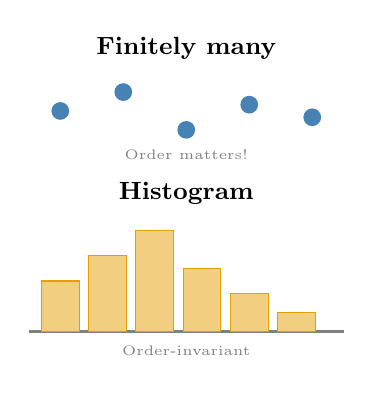
\begin{tikzpicture}[scale=0.8]
    % Finitely many agents
    \node[font=\small\bfseries] at (2.5,4.5) {Finitely many};
    \foreach \x/\y in {0.5/3.5, 1.5/3.8, 2.5/3.2, 3.5/3.6, 4.5/3.4} {
        \fill[softblue] (\x,\y) circle (4pt);
    }
    \node[font=\tiny, gray] at (2.5,2.8) {Order matters!};

    % Histogram
    \node[font=\small\bfseries] at (2.5,2.2) {Histogram};
    \draw[thick, gray] (0,0) -- (5,0);
    \foreach \x/\h in {0.5/0.8, 1.25/1.2, 2.0/1.6, 2.75/1.0, 3.5/0.6, 4.25/0.3} {
        \draw[fill=softorange!50, draw=softorange] (\x-0.3,0) rectangle (\x+0.3,\h);
    }
    \node[font=\tiny, gray] at (2.5,-0.3) {Order-invariant};
\end{tikzpicture}
\end{center}
\end{columns}
\end{frame}

% --- Slide 44: Neural Network Architecture ---
\begin{frame}{Neural Network Architecture}
\begin{center}
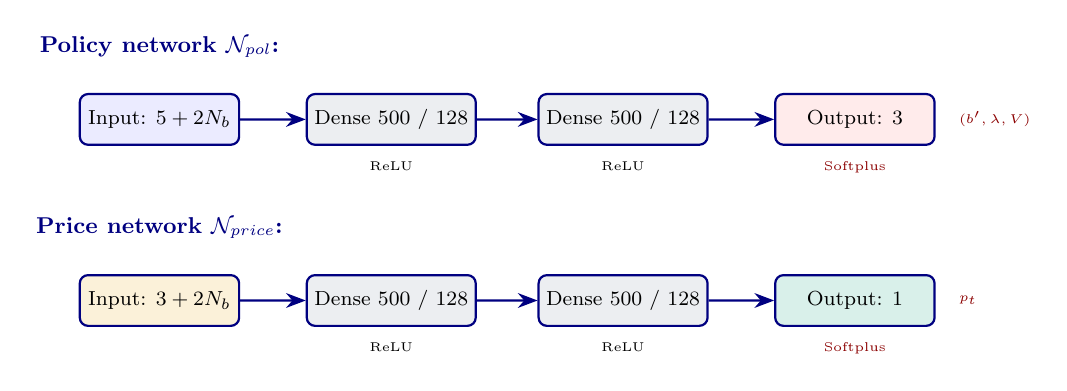
\begin{tikzpicture}[scale=0.92, every node/.style={transform shape},
    layer/.style={rectangle, draw=uzhblue, thick, fill=uzhgreylight,
        minimum width=2.2cm, minimum height=0.7cm, font=\footnotesize,
        rounded corners=3pt, inner sep=3pt},
    arr/.style={-{Stealth[length=2.5mm]}, thick, uzhblue}
]
    % Policy network
    \node[font=\small\bfseries, uzhblue] at (0,2.0) {Policy network $\mathcal{N}_{pol}$:};
    \node[layer, fill=blue!8] (pin) at (0,1.0) {Input: $5 + 2N_b$};
    \node[layer] (ph1) at (3.2,1.0) {Dense 500 / 128};
    \node[layer] (ph2) at (6.4,1.0) {Dense 500 / 128};
    \node[layer, fill=red!8] (pout) at (9.6,1.0) {Output: 3};

    \draw[arr] (pin) -- (ph1);
    \draw[arr] (ph1) -- (ph2);
    \draw[arr] (ph2) -- (pout);

    \node[below=0.1cm, font=\tiny] at (ph1.south) {ReLU};
    \node[below=0.1cm, font=\tiny] at (ph2.south) {ReLU};
    \node[below=0.1cm, font=\tiny, darkred] at (pout.south) {Softplus};
    \node[right=0.2cm, font=\tiny, darkred] at (pout.east) {$(b', \lambda, V)$};

    % Price network
    \node[font=\small\bfseries, uzhblue] at (0,-0.5) {Price network $\mathcal{N}_{price}$:};
    \node[layer, fill=softorange!15] (qin) at (0,-1.5) {Input: $3 + 2N_b$};
    \node[layer] (qh1) at (3.2,-1.5) {Dense 500 / 128};
    \node[layer] (qh2) at (6.4,-1.5) {Dense 500 / 128};
    \node[layer, fill=softgreen!15] (qout) at (9.6,-1.5) {Output: 1};

    \draw[arr] (qin) -- (qh1);
    \draw[arr] (qh1) -- (qh2);
    \draw[arr] (qh2) -- (qout);

    \node[below=0.1cm, font=\tiny] at (qh1.south) {ReLU};
    \node[below=0.1cm, font=\tiny] at (qh2.south) {ReLU};
    \node[below=0.1cm, font=\tiny, darkred] at (qout.south) {Softplus};
    \node[right=0.2cm, font=\tiny, darkred] at (qout.east) {$p_t$};
\end{tikzpicture}
\end{center}

\vspace{0.3em}
\begin{itemize}\small\itemsep1pt
    \item \textbf{Policy net:} individual + aggregate state $\to (b', \lambda, V)$
    \item \textbf{Price net:} aggregate state only $\to p$
    \item Softplus keeps outputs \emphc{strictly positive}
    \item Paper: 500 hidden units. Teaching notebook: 128.
    \item Both nets are trained \emphc{jointly} on equilibrium residuals
\end{itemize}
\end{frame}

% --- Slide 44: Equilibrium Conditions as Loss ---
\begin{frame}{Equilibrium Conditions as Loss}
\small
The DEQN solves \emphc{all equilibrium conditions simultaneously} (unsupervised):

\vspace{0.2em}
\begin{enumerate}\itemsep0pt
    \item \textbf{Euler equation (EE):} intertemporal optimality condition
    \vspace{-0.3em}
    \[
    \text{EE}: \quad \frac{\left(\frac{\beta \cdot \mathbb{E}_t[\cdots] + \lambda_t}{p_t}\right)^{-1/\rho}}{c_t} - 1 = 0
    \]
    \vspace{-0.5em}

    \item \textbf{Bellman equation (BE):} value function consistency
    \vspace{-0.3em}
    \[
    \text{BE}: \quad \frac{V^{opt}}{V^{net}} - 1 = 0
    \]
    \vspace{-0.5em}

    \item \textbf{Market clearing (MC):} aggregate bond demand $=$ supply
    \vspace{-0.3em}
    \[
    \text{MC}: \quad \left|\sum_{\eta} \sum_{j=1}^{N_b} h_t(\eta, b_j) \cdot b'(\eta, b_j, x_t^{agg}) - \bar B\right| = 0
    \]
    \vspace{-0.5em}

    \item \textbf{KKT complementarity:} $\lambda_t \cdot b_{t+1} = 0$

    \item \textbf{Consumption positivity:} $c_t > 0$ (penalty for violations)
\end{enumerate}
\end{frame}

% --- Slide 45: Euler Equation with Epstein-Zin ---
\begin{frame}{Loss: Euler and Bellman Equations with Epstein--Zin}
\small

\begin{block}{$V^{opt}$ (Bellman residual: $\text{BE} = V^{opt}/V^{net} - 1$)}
\vspace{-2pt}
\[
V^{opt}_t = \!\left[(1-\beta)\,c_t^{1-\rho} + \beta\,\chi_t^{1-\rho}\right]^{\!\frac{1}{1-\rho}},\quad
\chi_t = \!\left(\sum_{a',\eta'}\pi_{a'|a}\pi_{\eta'|\eta}V_{t+1}^{1-\sigma}\right)^{\!\frac{1}{1-\sigma}}
\]
\vspace{-4pt}
{\footnotesize $V_{t+1}$: price network at next-period state; $c_t$ from budget constraint.}
\end{block}

\vspace{0.15em}
\textbf{Euler expectation:}
\[
\mathbb{E}_t[\cdots] = \sum_{(a',\eta')} \pi_{a'|a}\pi_{\eta'|\eta}\, c_{t+1}^{-\rho} \left(\frac{V_{t+1}}{\chi_t}\right)^{\!\rho - \sigma}
\]

\vspace{0.1em}
\textbf{Relative Euler error} (sums over all $6 \times 2 = 12$ next-period shock combinations):
\[
\boxed{\text{EE} = \frac{\left(\frac{\beta \cdot \mathbb{E}_t[\cdots] + \lambda_t}{p_t}\right)^{-1/\rho}}{c_t} - 1}
\]
\end{frame}

% --- Slide 46: Market Clearing via Histogram ---
\begin{frame}{Loss: Market Clearing via Histogram}
\textbf{Key:} Young's histogram enables \emphc{exact aggregation}. No Monte Carlo needed.

\vspace{0.2em}
\[
\boxed{\text{MC} = \left|\sum_{\eta \in \{0.8, 1.2\}} \sum_{j=1}^{N_b} h_t(\eta, b_j) \cdot b'\!(\eta, b_j, x_t^{agg}) - \bar B\right|}
\]

\vspace{0.2em}
\begin{itemize}\itemsep1pt
    \item $h_t(\eta, b_j)$: mass at grid point $b_j$ with shock $\eta$
    \item $b'(\eta, b_j, x_t^{agg})$: savings policy from the neural network
    \item \emphc{Aggregate demand} $= \mathbf{h}_t \cdot \mathbf{b}'$ (dot product; exact, no MC noise)
    \item Equilibrium: total demand $= \bar B$; in the notebook $\bar B=1$ (\emphc{unit net supply})
\end{itemize}

\vspace{0.2em}
\begin{alertblock}{Implementation}
\small
The policy network is called on all $2N_b$ grid points $(\eta,b_j)$ with current $x_t^{agg}$.
Aggregate demand $= \mathbf{h}_t \cdot \mathbf{b}'$ is a dot product. Bonds are in net supply $\bar B$, normalized to \emphc{one} in the notebook.\\[1pt]
{\footnotesize Code: \texttt{aggdem = tf.reduce\_sum(h * b\_prime\_grid, axis=1)} $\approx 1$.}
\end{alertblock}
\end{frame}

% --- Slide 47: Combined Loss ---
\begin{frame}{Combined Loss Function}
\small
\textbf{Total loss} (sum of squared residuals):
\[
\boxed{\mathcal{L} = \frac{1}{N} \sum_{i=1}^{N} \left[\text{EE}_i^2 + \text{BE}_i^2 + (n_Z \cdot \text{MC}_i)^2 + \text{KKT}_i^2 + \text{CB}_i^2\right]}
\]

\vspace{0.1em}
\begin{center}
\begin{tabular}{lll}
\toprule
\textbf{Term} & \textbf{Condition} & \textbf{Interpretation} \\
\midrule
$\text{EE}^2$ & Euler equation & Intertemporal optimality \\
$\text{BE}^2$ & Bellman equation & Value function consistency \\
$\text{MC}^2$ & Market clearing & Bond market equilibrium \\
$\text{KKT}^2$ & $\lambda \cdot b' = 0$ & Borrowing constraint complementarity \\
$\text{CB}^2$ & $c > 0$ & Budget feasibility penalty \\
\bottomrule
\end{tabular}
\end{center}

\vspace{0.1em}
\begin{itemize}\footnotesize\itemsep0pt
    \item All residuals should be \emphc{zero} in equilibrium
    \item $n_Z$ scaling on MC: ensures comparable magnitude across terms
    \item Minimizing $\mathcal{L}$ finds an \emphc{approximate competitive equilibrium}
\end{itemize}
\end{frame}

% --- Slide 48: Young's Method Inside the DEQN Loop ---
\begin{frame}{Young's Method Inside the DEQN Training Loop}
\begin{center}
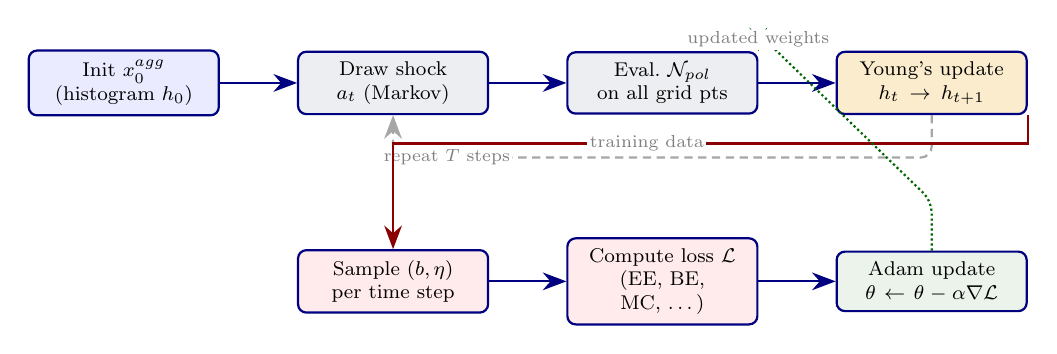
\begin{tikzpicture}[scale=0.9, every node/.style={transform shape},
    box/.style={rectangle, draw=uzhblue, thick, fill=uzhgreylight,
        minimum width=2.4cm, minimum height=0.8cm, font=\footnotesize,
        rounded corners=3pt, inner sep=4pt, text width=2.4cm, align=center},
    arr/.style={-{Stealth[length=3mm]}, thick, uzhblue},
    lbl/.style={font=\scriptsize, text=gray, fill=white, inner sep=1pt}
]
    % === Top row: Episode simulation ===
    \node[box, fill=blue!8] (start) at (0,0) {Init $x_0^{agg}$\\(histogram $h_0$)};
    \node[box] (shock) at (3.8,0) {Draw shock\\$a_t$ (Markov)};
    \node[box] (policy) at (7.6,0) {Eval.\ $\mathcal{N}_{pol}$\\on all grid pts};
    \node[box, fill=softorange!20] (young) at (11.4,0) {Young's update\\$h_t \to h_{t+1}$};

    \draw[arr] (start) -- (shock);
    \draw[arr] (shock) -- (policy);
    \draw[arr] (policy) -- (young);

    % Loop back arrow (cleaner routing)
    \draw[arr, densely dashed, gray!70, rounded corners=4pt]
        (young.south) -- ++(0,-0.6) -| (shock.south)
        node[lbl, pos=0.45] {repeat $T$ steps};

    % === Bottom row: Training ===
    \node[box, fill=red!8] (sample) at (3.8,-2.8) {Sample $(b,\eta)$\\per time step};
    \node[box, fill=red!8] (loss) at (7.6,-2.8) {Compute loss $\mathcal{L}$\\(EE, BE, MC, \ldots)};
    \node[box, fill=darkgreen!8] (update) at (11.4,-2.8) {Adam update\\$\theta \leftarrow \theta - \alpha\nabla\mathcal{L}$};

    \draw[arr, darkred] (young.south east) -- ++(0,-0.4) -| (sample.north)
        node[lbl, pos=0.3] {training data};
    \draw[arr] (sample) -- (loss);
    \draw[arr] (loss) -- (update);

    % Feedback arrow from update back to policy
    \draw[arr, darkgreen, densely dotted, rounded corners=4pt]
        (update.north) -- ++(0,0.7) -- (policy.south east |- 0,0.7) -- (policy.north east)
        node[lbl, pos=0.35] {updated weights};
\end{tikzpicture}
\end{center}

\vspace{0.1em}
{\small The histogram evolves \emphc{during training}: the network adapts to the equilibrium distribution.}
\end{frame}

% --- Slide 49: Histogram Update in TensorFlow ---
\begin{frame}[fragile]{Distribution Update in TensorFlow}
\begin{center}
\begin{minipage}{0.92\textwidth}
\begin{lstlisting}[basicstyle=\tiny\ttfamily, breaklines=true]
def get_weights_grid(asearch, agrid, deltaa):
    """Interpolation weights for Young's method."""
    dif = tf.abs(agrid - asearch)
    mask = tf.cast(dif < deltaa, tf.float32)
    w = (1.0 - dif / deltaa) * mask
    w = w / tf.reduce_sum(w, axis=1, keepdims=True)
    return w

def get_weights_eta(net_pol, X_agg):
    """Full histogram update using policy network."""
    h_new = tf.zeros_like(h)
    for eta_idx in range(n_eta):
        b_next = net_pol(eta, grid, X_agg)[:, 0:1]
        weights_next = get_weights_grid(b_next, agrid, deltaa)
        for eta_next in range(n_eta):
            h_new[eta_next] += pi_eta[eta_idx, eta_next] \
                             * (h[eta_idx] @ weights_next)
    h_new = normalize_per_eta(h_new, nA, target_mass=0.5)
    return h_new
\end{lstlisting}
\end{minipage}
\end{center}

\vspace{-0.2em}
{\footnotesize \texttt{get\_weights\_grid}: interpolation weights.\\
\texttt{normalize\_per\_eta}: keeps each $\eta$ block at mass 0.5.}
\end{frame}

% --- Slide 50: Episode-Based Training ---
\begin{frame}{Episode-Based Training}
\begin{block}{Training Algorithm}
\begin{algorithmic}
\scriptsize
\STATE \textbf{Input:} Networks $\mathcal{N}_{pol}$, $\mathcal{N}_{price}$; Adam optimizer ($\alpha = 10^{-5}$)
\STATE Initialize histogram: equal mass at a single grid point
\FOR{episode $= 1, \ldots, N_{\text{ep}}$}
    \STATE 1. Simulate aggregate shocks for $T$ steps
    \STATE 2. Propagate histogram via Young's method using current $\mathcal{N}_{pol}$
    \STATE 3. For each $t$: sample random $(b, \eta)$ pairs as idiosyncratic states
    \STATE 4. Form training batch: $\{(x_t^{id}, x_t^{agg}, x_{t+1}^{agg})\}$
    \STATE 5. Train for 1 epoch (batch size $= 128$, Adam)
    \STATE 6. Update starting histogram from end of simulation
\ENDFOR
\end{algorithmic}
\end{block}

\vspace{0.1em}
{\small Notebook modes: smoke $(N_{\text{ep}}=100,\,T=256)$, classroom $(500,\,256)$, production $(65{,}000,\,2048)$.}
\end{frame}

\begin{frame}{Training Design Choices}
\small
\begin{columns}[T]
\column{0.48\textwidth}
\begin{block}{Why episode-based training?}
\begin{itemize}\itemsep3pt
    \item The policy network changes the next histogram
    \item The next histogram changes prices and market clearing
    \item So the distribution must \emphc{co-evolve} with the network
\end{itemize}
\end{block}

\column{0.48\textwidth}
\begin{block}{Practical implementation}
\begin{itemize}\itemsep3pt
    \item Default notebook mode is \emphc{smoke} so the full pipeline runs during class
    \item Carry the ending histogram into the next episode
    \item Use several parallel tracks for diverse starting points
    \item Check diagnostics on actual simulated states, not schematic plots
\end{itemize}
\end{block}
\end{columns}
\end{frame}

\begin{frame}{How to Evaluate a Real Training Run}
\small
\begin{block}{Do not use schematic plots}
Diagnostics should come from \emphc{actual notebook output} or from \emphc{paper-reported tables and figures}, not from hand-drawn convergence shapes.
\end{block}

\vspace{0.3em}
\begin{columns}[T]
\column{0.32\textwidth}
\textbf{1.\ Residuals}
\begin{itemize}\itemsep2pt
    \item Euler residuals
    \item Market-clearing residuals
    \item KKT / Bellman terms
\end{itemize}

\column{0.32\textwidth}
\textbf{2.\ Policy checks}
\begin{itemize}\itemsep2pt
    \item Monotonicity in wealth
    \item Borrowing limit respected
    \item Sensible response to income
\end{itemize}

\column{0.32\textwidth}
\textbf{3.\ Distribution checks}
\begin{itemize}\itemsep2pt
    \item Histogram remains normalized
    \item Mean evolves plausibly
    \item Prices clear given the histogram
\end{itemize}
\end{columns}
\end{frame}

\begin{frame}{Why Young's Method Matters Inside DEQNs}
\small
\begin{block}{The role of Young's method in a DEQN}
\begin{enumerate}\itemsep1pt
    \item \emphc{Finite-dimensional encoding} of the distribution.
    \item \emphc{Differentiable} forward simulation (backprop-compatible).
    \item \emphc{Exact market clearing} computed from the histogram dot product.
    \item The policy network is evaluated on the \emphc{full $2\!\times\!N_b$ grid}, not just on sampled training states.
\end{enumerate}
\end{block}

\vspace{0.3em}
\begin{alertblock}{Takeaway}
The DEQN does not replace the distributional law of motion.  Young's method remains the device that turns individual decisions into an aggregate state that can be differentiated through.
\end{alertblock}
\end{frame}

\begin{frame}{Where Are We?}
\begin{enumerate}
    \item \textcolor{gray}{Motivation: Why Track Distributions?} \checkmark
    \vspace{0.25em}
    \item \textcolor{gray}{Young's (2010) Non-Stochastic Simulation} \checkmark
    \vspace{0.25em}
    \item \textcolor{gray}{KS benchmark + teaching-model switch} \checkmark
    \vspace{0.25em}
    \item \textcolor{gray}{DEQN teaching implementation} \checkmark
    \vspace{0.25em}
    \item \emphc{$\Rightarrow$ Alternative deep-learning approaches to KS}
\end{enumerate}
\end{frame}

% ============================================================================
% PART V: ALTERNATIVE DEEP-LEARNING APPROACHES TO KRUSELL--SMITH
% ============================================================================

% --- Part V divider ---
\begin{frame}{}
\vfill
\begin{center}
{\Huge \textcolor{uzhblue}{\textbf{Part V}}}\\[12pt]
{\LARGE Alternative Deep-Learning Approaches to Krusell--Smith}
\end{center}
\vfill
\end{frame}

% --- Slide: Three DL Recipes ---
\begin{frame}{Three Deep-Learning Recipes for KS}
\small
All three recipes minimize residuals of the \emph{same} structural equations via SGD.  They differ in how the aggregate distribution is fed to the network.

\vspace{0.4em}
\begin{center}
\scriptsize
\begin{tabular}{p{2.8cm} p{3.2cm} p{2.8cm} p{3.0cm}}
\toprule
 & \textbf{Histogram DEQN} & \textbf{All-in-one DL} & \textbf{DeepHAM} \\
 & (this lecture so far) & Maliar--Maliar--Winant & Han--Yang--E \\
\midrule
Distribution input & fixed-grid histogram vector & explicit $N$-agent panel & learned generalized moments \\
\addlinespace
Input dimension & $\mathcal{O}(N_b)$ & $\mathcal{O}(N)$ & $M \ll N_b$ (learned) \\
\addlinespace
Permutation invariance & automatic & approximate (LLN) & \emphc{architectural} (DeepSets) \\
\addlinespace
Main reference & Azinovic et al.\ (2022) & Maliar, Maliar \& Winant (2021) & Han, Yang \& E (2023) \\
\bottomrule
\end{tabular}
\end{center}

\vspace{0.3em}
{\footnotesize The accompanying notebook \texttt{12\_KrusellSmith\_DeepLearning.ipynb} implements the middle column at classroom scale.}
\end{frame}

% --- Slide: All-in-One DL (Part 1 of 2) ---
\begin{frame}{All-in-One Deep Learning (Maliar, Maliar \& Winant 2021)}
\small
\textbf{Idea.}  Cast every equilibrium condition as a \emph{residual that should vanish}, and train deep networks by minimizing the squared residual on simulated paths.

\vspace{0.4em}
\begin{block}{Loss components (for Krusell--Smith)}
\footnotesize
\begin{itemize}\itemsep1pt
    \item \textbf{Euler residual:} $\mathrm{EE} = u'(c_t) - \beta\,\E{u'(c_{t+1}) R_{t+1}}$, Monte Carlo over next-period shocks.
    \item \textbf{Bellman residual} on an auxiliary value network.
    \item \textbf{Market clearing:} $\sum_{i=1}^N k_{t+1}^i = N\bar K_{t+1}$.
    \item \textbf{Borrowing constraint:} softplus on savings head or Fischer--Burmeister residual.
\end{itemize}
\end{block}

\vspace{0.4em}
{\scriptsize Reference: Maliar, Maliar \& Winant (2021), \emph{J.\ Monet.\ Econ.}\ 122, 76--101.}
\end{frame}

% --- Slide: All-in-One DL (Part 2 of 2) ---
\begin{frame}{All-in-One DL: Scale and Replication}
\small
\textbf{Scale reported by the authors.}
\begin{itemize}\itemsep1pt
    \item Up to $N = 10{,}000$ explicit agents.
    \item State dimension $2{,}001+$ (one per agent plus aggregate).
    \item Approximation errors below $1\%$ on consumption-saving.
\end{itemize}

\vspace{0.4em}
\textbf{Replication code.}\\
\texttt{github.com/marcmaliar/deep-learning-euler-method-krusell-smith}

\vspace{0.4em}
\textbf{In this course.}  Notebook \texttt{12\_KrusellSmith\_DeepLearning.ipynb} is a classroom-scale caricature of this approach: single policy network, panel of $N \sim 100$ agents, CPU-friendly,  to convergence.
\end{frame}

% --- Slide: DeepHAM (Part 1 of 2) ---
\begin{frame}{DeepHAM --- Learned Moments (Han, Yang \& E)}
\small
\textbf{Idea.}  Instead of tracking the histogram or committing to the first moment \emph{a priori}, \emphc{learn} which summary statistics agents actually need.

\vspace{0.4em}
\begin{block}{Generalized moments via DeepSets}
\footnotesize
\begin{equation*}
\bm{m}_t = \Bigl(\textstyle\sum_i g_\theta^1(s_t^i),\; \ldots,\; \sum_i g_\theta^M(s_t^i)\Bigr), \qquad M \ll N_b
\end{equation*}
Each $g_\theta^m:\R^d\!\to\!\R$ is a neural encoder trained \emph{jointly} with the value and policy networks.  Sum-pooling $\Rightarrow$ permutation invariance.
\end{block}

\vspace{0.4em}
{\scriptsize Reference: Han, Yang \& E (2024), \emph{Quantitative Economics} (forthcoming); preprint arXiv:2112.14377.}
\end{frame}

% --- Slide: DeepHAM (Part 2 of 2) ---
\begin{frame}{DeepHAM: Reported Accuracy and Extensions}
\small
\textbf{Results on baseline KS:}
\begin{itemize}\itemsep2pt
    \item First moment only: Bellman error reduced by $37.5\%$ vs.\ classical KS.
    \item With one \emph{learned} moment: Bellman error reduced by $54.2\%$.
\end{itemize}

\vspace{0.6em}
\textbf{Extensions where DeepHAM shines.}
\begin{itemize}\itemsep2pt
    \item Multiple endogenous states (capital + bonds).
    \item Large aggregate shocks (risky steady state).
    \item Zero lower bound; occasionally binding constraints that bite on a non-trivial mass.
\end{itemize}

\vspace{0.6em}
{\scriptsize These are settings where both classical KS and the local perturbation method of Reiter (2009) break down.}
\end{frame}

% --- Slide: Comparison head-to-head ---
\begin{frame}{Head-to-Head: When to Use Which?}
\footnotesize
\begin{center}
\begin{tabular}{p{3.2cm} p{3.6cm} p{3.6cm}}
\toprule
 & \textbf{Pros} & \textbf{When it shines} \\
\midrule
\textbf{Histogram DEQN} (Azinovic et al., 2022) & Interpretable state; exact market clearing; DEQN-template reuse & Teaching; $N_b$ moderate; smooth policies \\
\addlinespace
\textbf{All-in-one DL} (Maliar, Maliar \& Winant, 2021) & No grid design; large-$N$ panels; single optimizer for all residuals & Large-$N$ research problems; OLG-many-cohort extensions \\
\addlinespace
\textbf{DeepHAM} (Han, Yang \& E, 2023) & Learned moments; risky steady state; ZLB; multiple endogenous states & Rich HA macro-finance with nonlinear aggregate effects \\
\bottomrule
\end{tabular}
\end{center}

\vspace{0.3em}
\begin{block}{Classical baseline}
\scriptsize
The canonical \emphc{traditional} KS implementation (\texttt{econ-ark/KrusellSmith} REMARK) achieves $R^2 > 0.9999$ in $\sim 20$ outer iterations on the baseline model.  All deep-learning methods aim to match or beat this, and to extend beyond the benchmark where KS can't.
\end{block}
\end{frame}

% --- Slide: Replication Codes ---
\begin{frame}{Replication Codes + Where to Get Them}
\scriptsize
\begin{center}
\begin{tabular}{p{3.3cm} p{7.5cm}}
\toprule
\textbf{Approach} & \textbf{Repository (on GitHub)} \\
\midrule
Traditional KS (baseline) & \texttt{econ-ark/KrusellSmith} \\
& \quad\emph{REMARK replication; forecasting-rule algorithm.} \\
\addlinespace
All-in-one DL (MMW 2021) & \texttt{marcmaliar/deep-learning-\allowbreak euler-method-\allowbreak krusell-smith} \\
& \quad\emph{TensorFlow implementation accompanying the JME paper.} \\
\addlinespace
Histogram DEQN & \texttt{sischei/DeepEquilibriumNets} \\
& \quad\emph{Azinovic, Gaegauf \& Scheidegger (2022) code.} \\
\addlinespace
Classroom MMW-style (this course) & \texttt{day4/code/\allowbreak 12\_KrusellSmith\_\allowbreak DeepLearning.ipynb} \\
& \quad\emph{Self-contained, CPU-friendly,  training.} \\
\addlinespace
DeepHAM & Authors' page; contact the authors for code. \\
\bottomrule
\end{tabular}
\end{center}
\end{frame}

% ============================================================================
% WRAP-UP
% ============================================================================

% --- Summary ---
\begin{frame}{Summary}
\scriptsize
\begin{block}{Key Messages}
\begin{enumerate}
    \item \textbf{HA models} require tracking the wealth distribution, an infinite-dimensional state variable.
    \item \textbf{Young (2010)} gives a deterministic histogram update: no Monte Carlo noise, exact mean preservation.
    \item \textbf{Krusell--Smith} is the benchmark layer: it explains approximate aggregation and the forecasting-rule loop.
    \item \textbf{Notebook 11} is the teaching-code layer: Appendix A.5 reuses Young's method inside a DEQN with policy and price networks.
    \item \textbf{Young + DEQN} keeps exact histogram aggregation while removing the separate KS regression step.
\end{enumerate}
\end{block}
\end{frame}

% --- References ---
\begin{frame}{Core References}
{\scriptsize
\begin{itemize}\itemsep0pt
    \item Azinovic, M., Gaegauf, L., \& Scheidegger, S.\ (2022). Deep equilibrium nets. \emph{Int.\ Econ.\ Rev.}\ 63(4), 1471--1525.
    \item Den Haan, W.\ (2010). Assessing the accuracy of the aggregate law of motion in models with heterogeneous agents. \emph{J.\ Econ.\ Dyn.\ Control} 34(1), 79--99.
    \item \emphc{Han, J., Yang, Y., \& E, W.\ (2024). DeepHAM: A global solution method for HA models with aggregate shocks.} \emph{Quant.\ Econ.}\ (forthcoming); arXiv:2112.14377.
    \item Krusell, P., \& Smith, A.A.\ (1998). Income and wealth heterogeneity in the macroeconomy. \emph{J.\ Polit.\ Econ.}\ 106(5), 867--896.
    \item \emphc{Maliar, L., Maliar, S., \& Winant, P.\ (2021). Deep learning for solving dynamic economic models.} \emph{J.\ Monet.\ Econ.}\ 122, 76--101.
    \item Maliar, L., Maliar, S., \& Valli, F.\ (2010). \emph{J.\ Econ.\ Dyn.\ Control} 34(1), 42--49.
    \item Reiter, M.\ (2009). Solving heterogeneous-agent models by projection and perturbation. \emph{J.\ Econ.\ Dyn.\ Control} 33(3), 649--665.
    \item Young, E.R.\ (2010). Solving the incomplete markets model with aggregate uncertainty \ldots \ \emph{J.\ Econ.\ Dyn.\ Control} 34(1), 36--41.
\end{itemize}
}

{\scriptsize Bold-face entries are the two alternative DL methods covered in Part V and in the reading PDFs in \texttt{day4/readings/}.}
\end{frame}

% --- Notebook Map ---
\begin{frame}{Discrete-time DEQN Notebook Map}
\footnotesize
\begin{columns}[T]
\column{0.48\textwidth}
\begin{block}{Core (Parts II--IV)}
\texttt{10\_Youngs\_Method\_Examples}\\[3pt]
\texttt{11\_Continuum\_of\_Agents\_DEQN}
\end{block}

\begin{block}{Alternative DL (Part V)}
\texttt{12\_KrusellSmith\_DeepLearning}\\
\quad All-in-one DL; classroom scale
\end{block}

\column{0.48\textwidth}
\begin{block}{Sequence-space extension}
\texttt{05\_SequenceSpace\_BrockMirman}\\[3pt]
\texttt{06\_SequenceSpace\_KrusellSmith}
\end{block}

\begin{block}{External reference code}
\texttt{econ-ark/KrusellSmith}\\[2pt]
\texttt{marcmaliar/}\\
\texttt{deep-learning-euler-method-krusell-smith}
\end{block}
\end{columns}

\vspace{0.3em}
{\footnotesize All notebooks are in the course repository.}
\end{frame}

% --- Slide 59: Questions ---
\begin{frame}{}
\begin{columns}[c]
\column{0.48\textwidth}
\begin{center}
{\Huge \textcolor{uzhblue}{\textbf{Questions?}}}

\vspace{1.0cm}
{\large Simon Scheidegger}\\[4pt]
{\small HEC, University of Lausanne}\\[4pt]
\url{https://sischei.github.io}

\vspace{0.6cm}
{\footnotesize Materials:\\\url{https://github.com/sischei/Deep_Learning_for_Solving_And_Estimating_Dynamic_Economic_Models}}
\end{center}

\column{0.48\textwidth}
\begin{center}
\textbf{Next up --- Toolkit and continuous-time block:}\\[6pt]
{\large Toolkit T1: Agentic Programming}\\[4pt]
{\small Using AI agents for research}\\[10pt]
{\footnotesize PINNs \& continuous-time HA\\
Surrogates \& GPs\\
Climate \& Deep UQ}
\end{center}
\end{columns}
\end{frame}

\end{document}
